%% file: template.tex = LaTeX template for article-like report 
%% init: sometime 1993
%% last: Feb  8 2015  Rob Rutten  Deil
%% site: http://www.staff.science.uu.nl/~rutte101/rrweb/rjr-edu/manuals/student-report/

%% First read ``latex-bibtex-simple-manual.txt'' at
%% http://www.staff.science.uu.nl/~rutte101/Report_recipe.html

%% Start your report production by copying this file into your XXXX.tex.
%% Small changes to the header part will make it an A&A or ApJ manuscript.

%%%%%%%%%%%%%%%%%%%%%%%%%%%%%%%%%%%%%%%%%%%%%%%%%%%%%%%%%%%%%%%%%%%%%%%%%%%%
\documentclass{aa}   %% Astronomy & Astrophysics style class
\usepackage{graphicx,natbib,url,twoopt}
\usepackage[varg]{txfonts}           %% A&A font choice
\usepackage{hyperref}                %% for pdflatex
%%\usepackage[breaklinks]{hyperref}  %% for latex+dvips
%%\usepackage{breakurl}              %% for latex+dvips
\usepackage{pdfcomment}              %% for popup acronym meanings
\usepackage{acronym}                 %% for popup acronym meanings

\hypersetup{
  colorlinks=true,   %% links colored instead of frames
  urlcolor=blue,     %% external hyperlinks
  linkcolor=red,     %% internal latex links (eg Fig)
}

\bibpunct{(}{)}{;}{a}{}{,}    %% natbib cite format used by A&A and ApJ

\pagestyle{plain}   %% undo the fancy A&A pagestyle 

%% Add commands to add a note or link to a reference
\makeatletter
\newcommand{\bibnote}[2]{\@namedef{#1note}{#2}}
\newcommand{\biblink}[2]{\@namedef{#1link}{#2}}
\makeatother

%% Commands to make citations ADS clickers and to add such also to refs
%% May 2014: they give error stops ("Illegal parameter number ..."}
%%   for plain latex with TeX Live 2013; the ad-hoc fixes added below let
%%   latex continue instead of stop within these commands.
%%   Please let me know if you know a better fix!
%%   No such problem when using pdflatex.
\makeatletter
 \newcommandtwoopt{\citeads}[3][][]{%
   \nonstopmode%              %% fix to not stop at error message in latex
   \href{http://adsabs.harvard.edu/abs/#3}%
        {\def\hyper@linkstart##1##2{}%
         \let\hyper@linkend\@empty\citealp[#1][#2]{#3}}%   %% Rutten, 2000
   \biblink{#3}{\href{http://adsabs.harvard.edu/abs/#3}{ADS}}%
   \errorstopmode}            %% fix to resume stopping at error messages 
 \newcommandtwoopt{\citepads}[3][][]{%
   \nonstopmode%              %% fix to not stop at error message in latex
   \href{http://adsabs.harvard.edu/abs/#3}%
        {\def\hyper@linkstart##1##2{}%
         \let\hyper@linkend\@empty\citep[#1][#2]{#3}}%     %% (Rutten 2000)
   \biblink{#3}{\href{http://adsabs.harvard.edu/abs/#3}{ADS}}%
   \errorstopmode}            %% fix to resume stopping at error messages
 \newcommandtwoopt{\citetads}[3][][]{%
   \nonstopmode%              %% fix to not stop at error message in latex
   \href{http://adsabs.harvard.edu/abs/#3}%
        {\def\hyper@linkstart##1##2{}%
         \let\hyper@linkend\@empty\citet[#1][#2]{#3}}%     %% Rutten (2000)
   \biblink{#3}{\href{http://adsabs.harvard.edu/abs/#3}{ADS}}%
   \errorstopmode}            %% fix to resume stopping at error messages 
 \newcommandtwoopt{\citeyearads}[3][][]{%
   \nonstopmode%              %% fix to not stop at error message in latex
   \href{http://adsabs.harvard.edu/abs/#3}%
        {\def\hyper@linkstart##1##2{}%
         \let\hyper@linkend\@empty\citeyear[#1][#2]{#3}}%  %% 2000
   \biblink{#3}{\href{http://adsabs.harvard.edu/abs/#3}{ADS}}%
   \errorstopmode}            %% fix to resume stopping at error messages 
\makeatother

%% Acronyms
\newacro{ADS}{Astrophysics Data System}
\newacro{NLTE}{non-local thermodynamic equilibrium}
\newacro{NASA}{National Aeronautics and Space Administration}

%% Add popups with meaning to acronyms 
%% NB: only show up in Adobe Reader and do not work with \input or \include
\gdef\acp#1{%
  \pdfmarkupcomment[markup=Underline,color={1 1 1},author={{#1}},opacity=0]%
  {{#1}}{{\acl{#1}}}}

%% Spectral species
\def\MgI{\ion{Mg}{I}}          %% A&A; for aastex use \def\MgI{\ion{Mg}{1}} 
\def\MgII{\ion{Mg}{II}}        %% A&A; for aastex use \def\MgII{\ion{Mg}{2}} 

%% Hyphenation
\hyphenation{Schrij-ver}       %% Dutch ij is a single character

%%%%%%%%%%%%%%%%%%%%%%%%%%%%%%%%%%%%%%%%%%%%%%%%%%%%%%%%%%%%%%%%%%%%%%%%%%%%
\begin{document}  

%% simple header.  Change into A&A or ApJ commands for those journals

\twocolumn[{%
\vspace*{4ex}
\begin{center}
  {\Large \bf Milestone 1: The background evolution of the universe}\\[4ex]
  {\large \bf Andreas Ellewsen}\\[4ex]
  %\begin{minipage}[t]{15cm}
  %      $^1$ Institute of theoretical astrophysics\\

  %  {\bf Abstract.} Here be dragons

  %\vspace*{2ex}
  %\end{minipage}
\end{center}
}]
%%%%%%%%%%%%%%%%%%%%%%%%%%%%%%%%%%%%%%%%%%%%%%%%%%%%%%%%%%%%%%%%%%%%%%%%%%%%
\section{Introduction}\label{sec:introduction}
%%%%%%%%%%%%%%%%%%%%%%%%%%%%%%%%%%%%%%%%%%%%%%%%%%%%%%%%%%%%%%%%%%%%%%%%%%%%
In this project I will follow the algorithm presented in Callin(2005). This is part one of four for this project.
The first part involves computing the expansion history of the universe, as well as looking at the evolution of the density of various matter and energy components.
I have chosen to make this first part compatible with the inclusion of neutrinos. 

To ease the development of this code, I have been provided with a skeleton code of the project. This code includes a variety of methods needed to solve the project.

%%%%%%%%%%%%%%%%%%%%%%%%%%%%%%%%%%%%%%%%%%%%%%%%%%%%%%%%%%%%%%%%%%%%%%%%%%%%
\section{Analytical solution}\label{sec:analytical}
%%%%%%%%%%%%%%%%%%%%%%%%%%%%%%%%%%%%%%%%%%%%%%%%%%%%%%%%%%%%%%%%%%%%%%%%%%%%

%%%%%%%%%%%%%%%%%%%%%%%%%%%%%%%%%%%%%%%%%%%%%%%%%%%%%%%%%%%%%%%%%%%%%%%%%%%%
\section{Results}\label{sec:simulate_analytic}
%%%%%%%%%%%%%%%%%%%%%%%%%%%%%%%%%%%%%%%%%%%%%%%%%%%%%%%%%%%%%%%%%%%%%%%%%%%%
 The $\Omega_x$ values indicate the relative density of a given component compared to the critical density of the universe. 
 The critical density being that which corresponds to the universe begin flat.
 Looking at the figure we see radiation dominating from the start together with neutrinos.
 This continues for some time until the dark matter component starts to rise.
 We see that this starts before the baryon component. This is good since that makes it possible for dark matter to form structures that that baryons can later fall into. The radiation and neutrinos die out, and at a later point vacuum energy shoots up. At the end we end up with approximately 70\% vacuum energy(dark energy?), 25\% dark matter, and 5\% baryons. This is exactly as it should be since we 
 \begin{figure}
  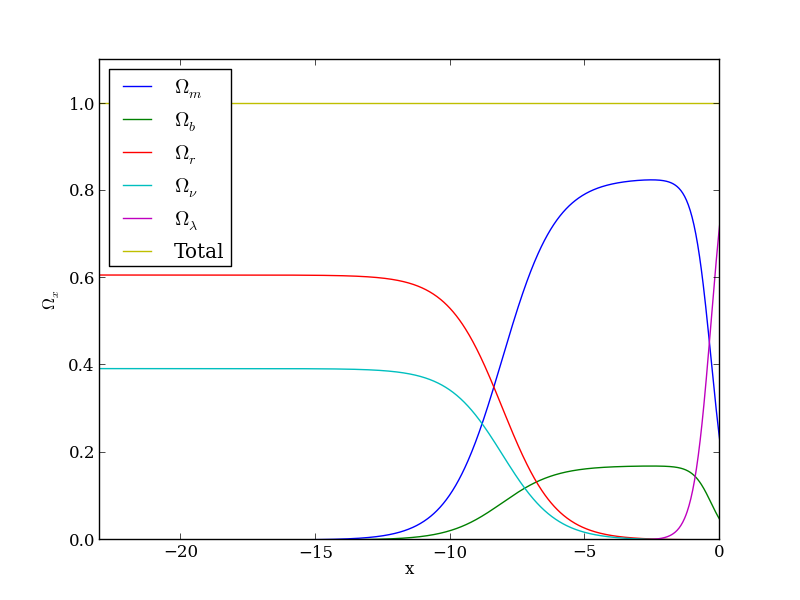
\includegraphics[width=.49\textwidth]{figure_0.png}
  \caption{}
 \label{figure0}
 \end{figure}
 
 Conformal time, detoneted by $\eta(x)$ measures the distance to the particle horizon for a given x value. A nice test of this is to insert the x-value of today.
 The answer should then be the radius of the observable universe. At the present this is measured to be approximately 14 billion parsecs (14Gpc). 
 The graph hits this value fairly well, indicating that everything is working properly so far. 
 Note also that there are in fact two graphs in this figure, one which is calculated from the differential equation for $\eta$. 
 And another one made by splining the first one and finding $\eta$ values at arbitrary values between those of the first function.
 
  \begin{figure}
  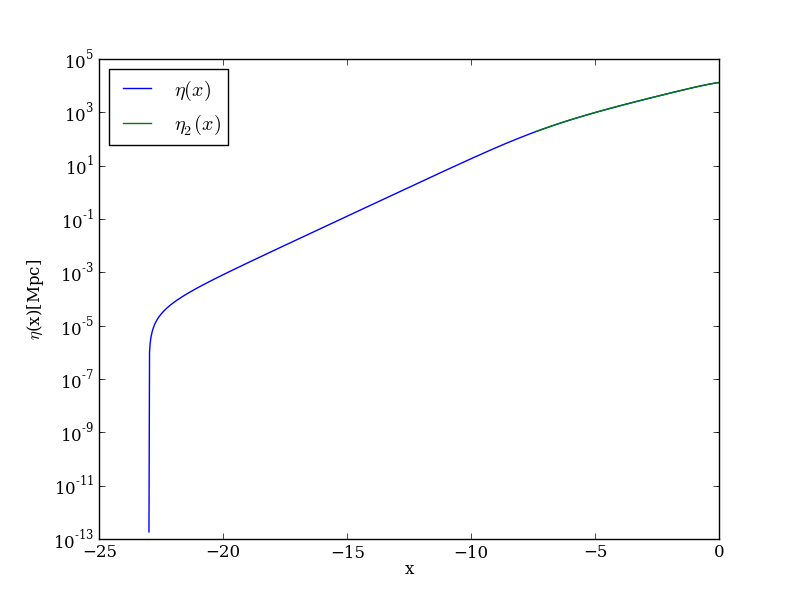
\includegraphics[width=.49\textwidth]{figure_1.png}
  \caption{}
 \label{figure1}
 \end{figure}
 
 The Hubble parameter $H$ is depicted both as a function of $x$, and $z$. Whether this is good or not is hard to say for the first part. We can at least put some faith in its correctness by the fact that it ends at $H_0 \approx 70$km s$^{-1}$Mpc$^{-1}$
 
  \begin{figure}
  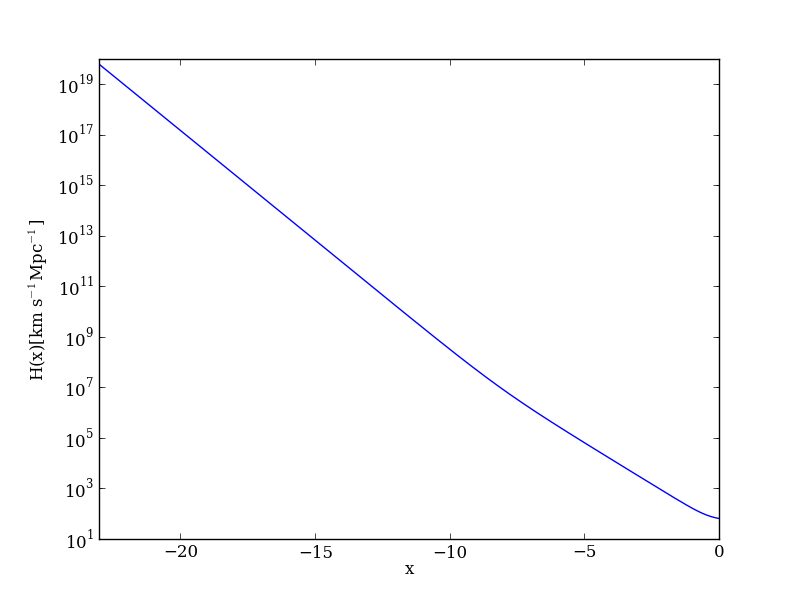
\includegraphics[width=.49\textwidth]{figure_2.png}
  \caption{}
 \label{figure2}
 \end{figure}

 
 \begin{figure}
  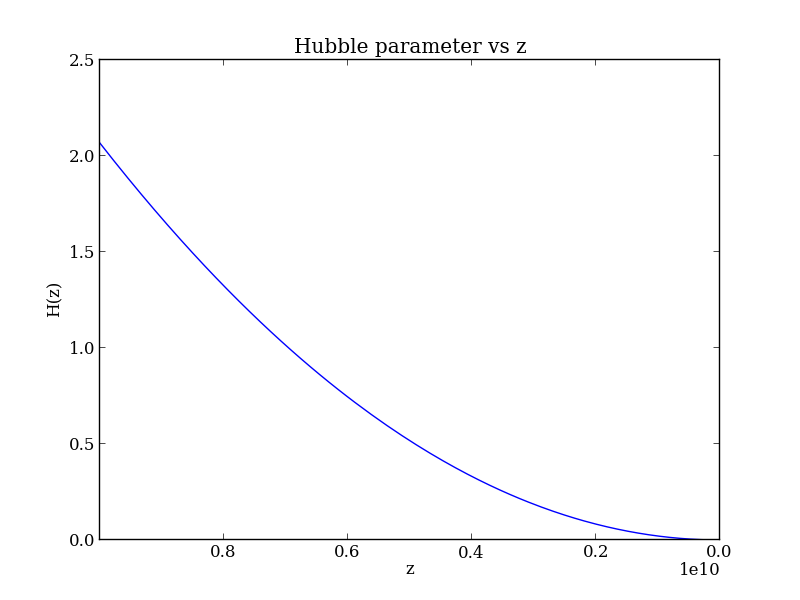
\includegraphics[width=.49\textwidth]{figure_3.png}
  \caption{}
 \label{figure3}
 \end{figure}
% 
% \begin{table}
%  \begin{tabular}{|c|c|c|}
%   \hline
%   &Analytical &Numerical \\
%   \hline
%   $<E>$ &-1.996 & -1.996\\
%   \hline
%   $<|M|>$& 0.999& 0.999\\
%   \hline
%   $C_V$ & 0.032& 0.032\\
%   \hline
%   $\chi$ & 0.004& 0.004\\
%   \hline
%  \end{tabular}
% \caption{Table of values from the analytical calculations for a system with L=2 and T = 1 in units of (kT/J). Note the precision of the numerical result.}
% \label{tab1}
% \end{table}

%%%%%%%%%%%%%%%%%%%%%%%%%%%%%%%%%%%%%%%%%%%%%%%%%%%%%%%%%%%%%%%%%%%%%%%%%%%%
\section{Conclusions} \label{sec:conclusions}
%%%%%%%%%%%%%%%%%%%%%%%%%%%%%%%%%%%%%%%%%%%%%%%%%%%%%%%%%%%%%%%%%%%%%%%%%%%%

%%%%%%%%%%%%%%%%%%%%%%%%%%%%%%%%%%%%%%%%%%%%%%%%%%%%%%%%%%%%%%%%%%%%%%%%%%%%
\section{Source code}\label{sec:files}
%%%%%%%%%%%%%%%%%%%%%%%%%%%%%%%%%%%%%%%%%%%%%%%%%%%%%%%%%%%%%%%%%%%%%%%%%%%%

%%%%%%%%%%%%%%%%%%%%%%%%%%%%%%%%%%%%%%%%%%%%%%%%%%%%%%%%%%%%%%%%%%%%%%%%%%%%
%\begin{acknowledgements}
%\end{acknowledgements}

%%%%%%%%%%%%%%%%%%%%%%%%%%%%%%%%%%%%%%%%%%%%%%%%%%%%%%%%%%%%%%%%%%%%%%%%%%%%
%% references
\section{References}
Itzhak Bars; John Terning (November 2009). Extra Dimensions in Space and Time. Springer. pp. 27

%\bibliographystyle{aa-note} %% aa.bst but adding links and notes to references
%\raggedright              %% only for adsaa with dvips, not for pdflatex
%\bibliography{XXX}          %% XXX.bib = your Bibtex entries copied from ADS

\end{document}